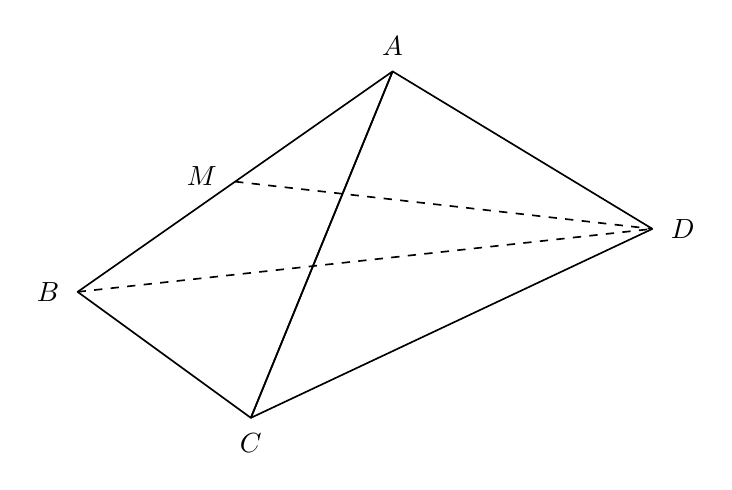
\begin{tikzpicture}[x=1cm,y=1cm,line width=.6pt,font=\normalsize,line join=round]
% tetrahedron ABCD, M midpoint of AB
\coordinate (A) at (1.2,3.2);
\coordinate (B) at (-2.8,0.4);
\coordinate (C) at (-0.6,-1.2);
\coordinate (D) at (4.5,1.2);
\coordinate (M) at (-0.8,1.8);
% faces: solid ABC, ACD; hidden BD, MD dashed
\draw (A)--(B)--(C)--cycle;
\draw (A)--(C);
\draw (A)--(D);
\draw (C)--(D);
\draw[dashed] (B)--(D);
\draw[dashed] (M)--(D);
% labels with clearance
\node[above,yshift=2pt] at (A) {$A$};
\node[left,xshift=-3pt] at (B) {$B$};
\node[below,yshift=-2pt] at (C) {$C$};
\node[right,xshift=3pt] at (D) {$D$};
\node[left,xshift=-3pt,yshift=2pt] at (M) {$M$};
\end{tikzpicture}
